\chapter{Calculando o Layout da Página com typearea}
Muitas classes \LaTeX, incluindo as classes padrão, apresentam ao usuário uma configuração amplamente fixa de margens e layout de página. Nas classes padrão, a escolha é limitada a selecionar um tamanho de fonte. Existem pacotes separados, como geometry, que dão ao usuário controle completo sobre, mas também total responsabilidade por, definir a área de tipo e margens.

O \KOMAScript\ adota uma abordagem um pouco diferente com o pacote typearea. Os usuários recebem maneiras de ajustar o design e os algoritmos com base em padrões tipográficos estabelecidos, tornando mais fácil para eles fazerem boas escolhas.

No LaTeX, o espaçamento entre linhas é definido em cerca de 20\% do tamanho da fonte.
Comprimentos de linha acima de 80 caracteres são inaceitáveis.

O \LaTeX\ reconhece os comandos \verb|\raggedbottom| e \verb|\flushbottom|. \verb|\raggedbottom| especifica que a última linha de uma página deve ser posicionada onde quer que tenha sido calculada. Isso significa que a posição desta linha pode ser diferente em cada página, até a altura de uma linha — ainda mais quando o fim da página coincide com títulos, figuras, tabelas ou similares. Em documentos frente e verso isso geralmente é indesejável. O segundo comando, \verb|\flushbottom|, garante que a última linha esteja sempre na borda inferior da área de texto. Para obter essa compensação vertical, o  \LaTeX\ pode ter que esticar a cola vertical além do que é normalmente permitido. O salto de parágrafo é uma cola vertical tão elástica, mesmo quando definido como zero. Para evitar esticar em páginas normais onde o espaçamento de parágrafo é a única cola elástica, a altura da área de texto deve ser um múltiplo da altura da linha de texto, incluindo a distância da primeira linha do topo da área de texto.

\section{Construindo a Área de Tipo por Divisão}
A maneira mais fácil de garantir que a área de texto tenha a mesma proporção da página é a seguinte:

 \begin{enumerate}
     \item Primeiro, subtraia o BCOR necessário para a correção de encadernação da borda interna do papel e divida o restante da página verticalmente em linhas DIV de altura igual.
     \item Em seguida, divida a página horizontalmente no mesmo número (DIV) de colunas de largura igual.
     \item Pegue a linha mais alta como a margem superior e as duas linhas mais baixas como a margem inferior. Se estiver imprimindo frente e verso, você também pega a coluna mais interna como a margem interna e as duas colunas mais externas como a margem externa.
     \item Adicione o BCOR de correção de encadernação à margem interna.
 \end{enumerate}
\bigskip
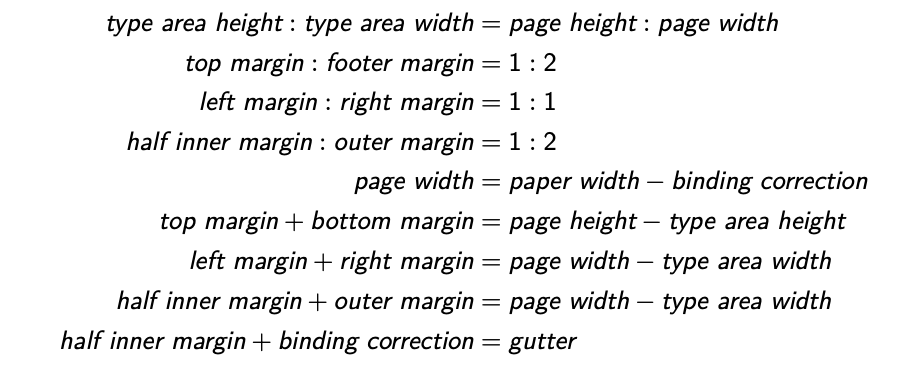
\includegraphics[scale=0.8]{imagem01.png}
